



























%%%%%%%%%%%%%%%%%%%%%%%%%%%%%%%%%%%%%%%%%%%%%%%%%%%%%%%%%%%%%%%%


\begin{comment}
	content...
	
	\subsection{Back-End}
	C’est le développement cote serveur c’est-à-dire la partie du code exécutée par le serveur.
\end{comment}



\subsubsection{Serveur Web : Amazon Web Services (AWS)}
Amazon Web Services (AWS) est la plateforme cloud la plus complète et la plus largement adoptée au monde. Elle propose plus de 200 services complets issus de centres de données du monde entier. Des millions de clients (dont certaines des startups les plus dynamiques au monde, de très grandes entreprises et des agences fédérales de premier plan) utilisent AWS pour réduire leurs coûts, gagner en agilité et innover plus rapidement.
\newline Pour en savoir plus, veillez
visiter le lien : \href{https://aws.amazon.com/fr/what-is-aws/#:~:text=Amazon%20Web%20Services%20(AWS)%20est,de%20donn%C3%A9es%20du%20monde%20entier.}{https://aws.amazon.com/fr/what-is-aws}


\subsection{Motifs d’architecture logicielle}
\subsubsection{MVC}

Ce figure ci-dessous résume en quelque sort le fonctionnement de
notre application.
L’api est considéré comme l’intermédiaire entre la partie données
(base de données) et la partie présentation (Application mobile).
\begin{figure}[h!]
	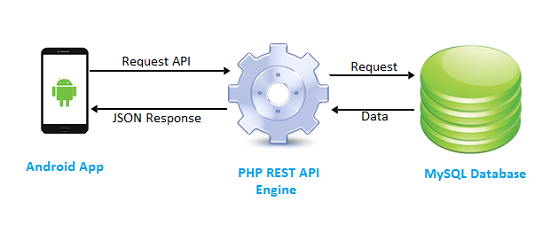
\includegraphics[width=15cm, height=8cm]{./Template LaTeX/Images/php-mysql-rest-api-for-android.png}
	\caption{PHP MySQL REST API pour Android}
	\label{fig:birds}
\end{figure}
\newline \newline \newline
